\documentclass[10pt,a4paper]{article}
\usepackage[latin1]{inputenc}
\usepackage{amsmath}
\usepackage{amsfonts}
\usepackage{amssymb}
\usepackage{clrscode}
\usepackage{graphicx}
\author{Wendy Moniuk - 996659343}
\title{CSC263 A4}
\begin{document}
\begin{enumerate}
\item
\begin{enumerate}
\item
My algorithm start by looping through the columns of the adjacency matrix until it finds a column of all ones, it then checks the corresponding row to see if it is all zeros except the one on the main diagonal.
\begin{codebox}
\Procname{$\proc{FindMovieStar}(A, n)$}
\li $\id{potStar} gets 0$
\li \For $j$ in $1\twodots n$
\li 	\Do
\li 	\If $\id{potStar} = 0$
\li		$\id{isStar} \gets \const{True}$
\li 	\For $i$ in $1\twodots n$
\li 	\Do
\li 		\If $A[i,j] = 0$
\li \Then
\li 	$\id{isStar} \gets \const{False}$
		\End
		\End
\li 	\If $\id{isStar} = \const{True}$ 
\li \Then
\li 	$\id{potStar} \gets j$
	\End
	\End
\li \If $\id{potStar} \neq 0$
\li \Then
\li \For $j$ in $1\twodots n$
\li \Do
\li 	\If $A[\id{potStar}, j] = 1 \bigwedge \id{potStar} \neq j$
\li 	\Then 
\li 		\Return 0	
		\End
\End
\End
\li \Return $\id{potStar}$

\end{codebox}

In order to check for a movie star the algorithm must see if everyone knows the movie star and the movie star knows nobody else. The first for loops check if there is a patron that everybody knows. The second loop inside the if statement takes that person and sees if they know anyone other than themselves. This algorithm relies on there only being one movie star which is true because of how a movie star is defined. If a movie star knows only themselves they cannot know another movie star in the bar, hence there is no other movie star.

\item
The worst case for my algorithm is that the last person we check is the movie star. In this case my algorithm takes $n^2 + n$ matrix accesses. 
$n^2$ for finding someone everyone knows and 
$n$ for checking that the person doesn't know anybody else.
\end{enumerate}
\item
\begin{enumerate}
\item See Figure 1.
\begin{figure}[htbp]
\centering
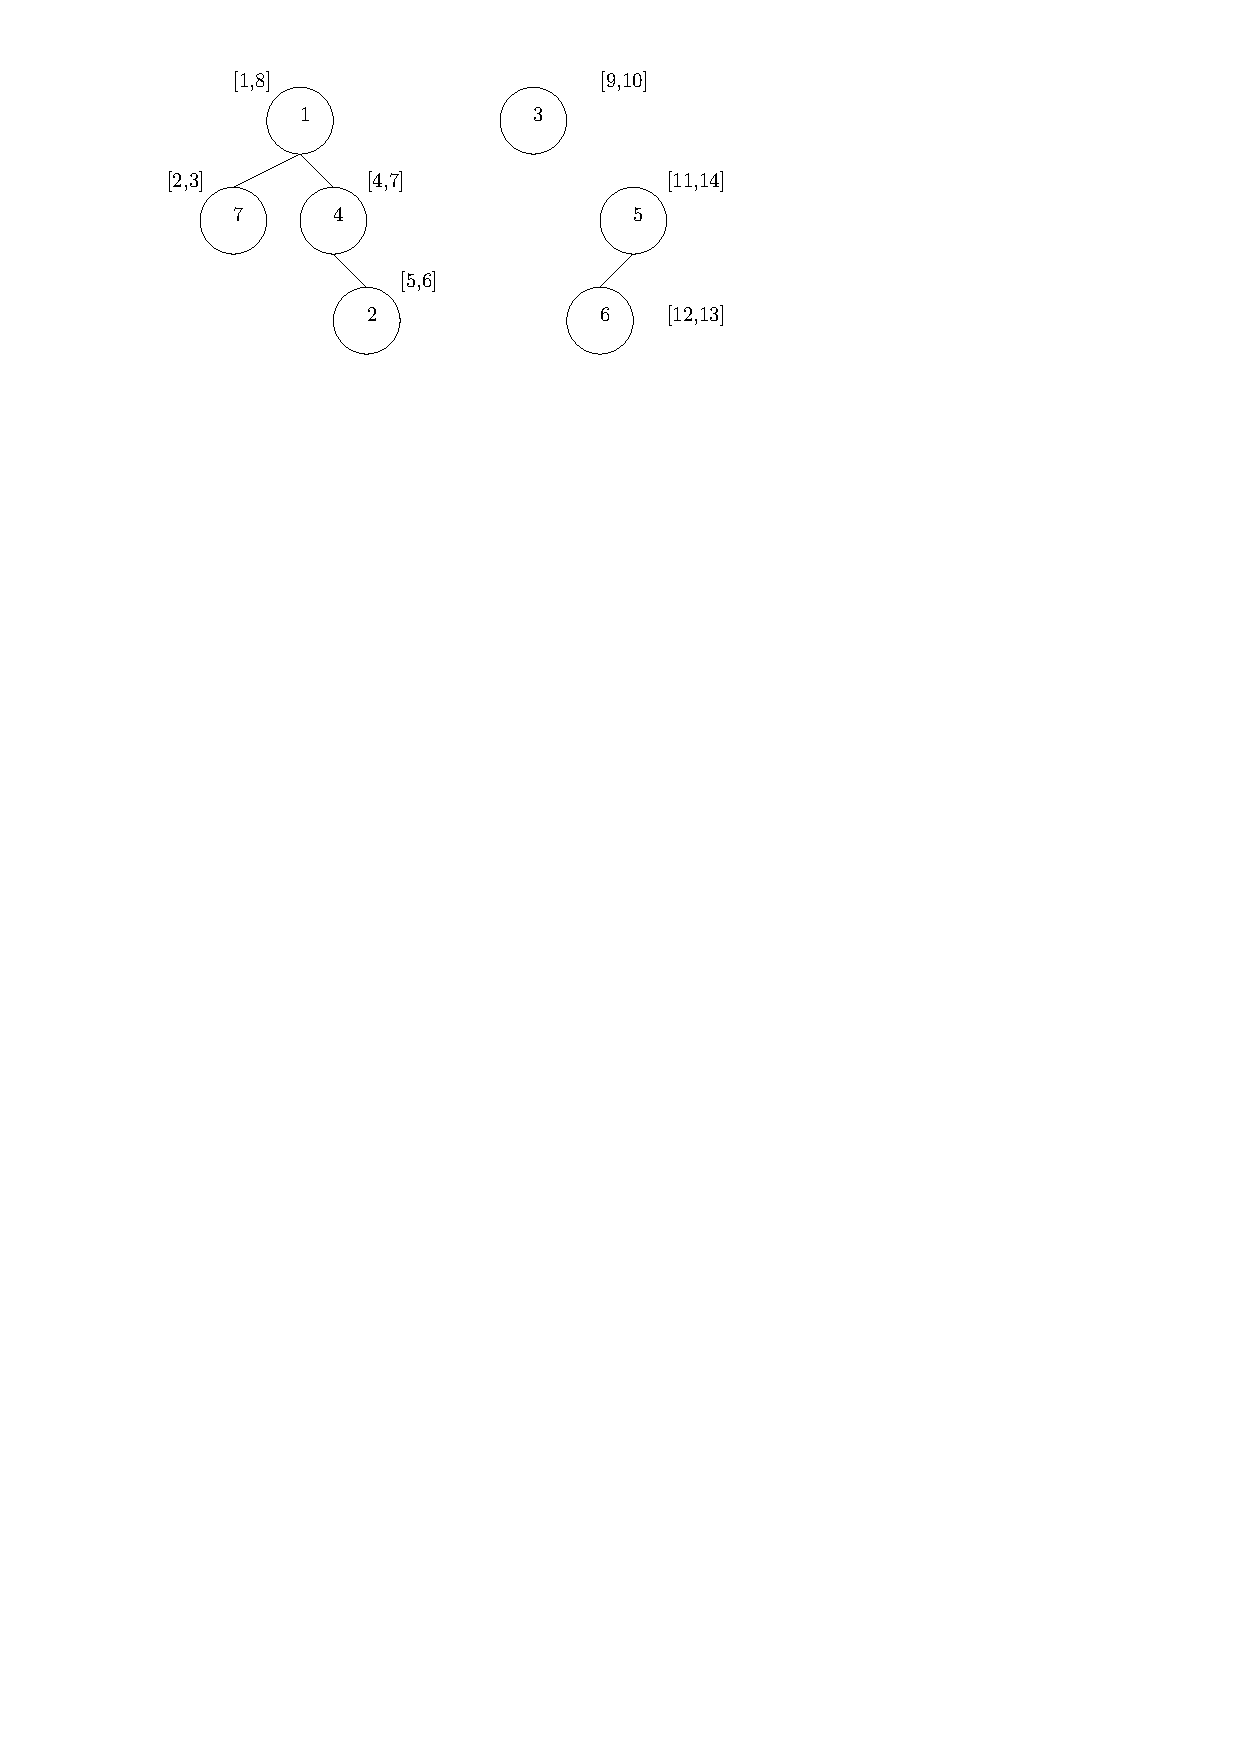
\includegraphics[width=\textwidth]{./A3Q2}
\caption{}
\label{fig:2a}
\end{figure}
\item
There are 10 cross edges, 1 forward edge and no back edges
\item There are no back edges and therefore no cycles. This means that no course can require itself and that there is an order that the courses can be taken in.
\item 5,6,3,1,4,2,7 using the topological sort from pg 613 in CLRS and the tutorial.
\item
See Figure 2
\begin{figure}[htbp]
\centering
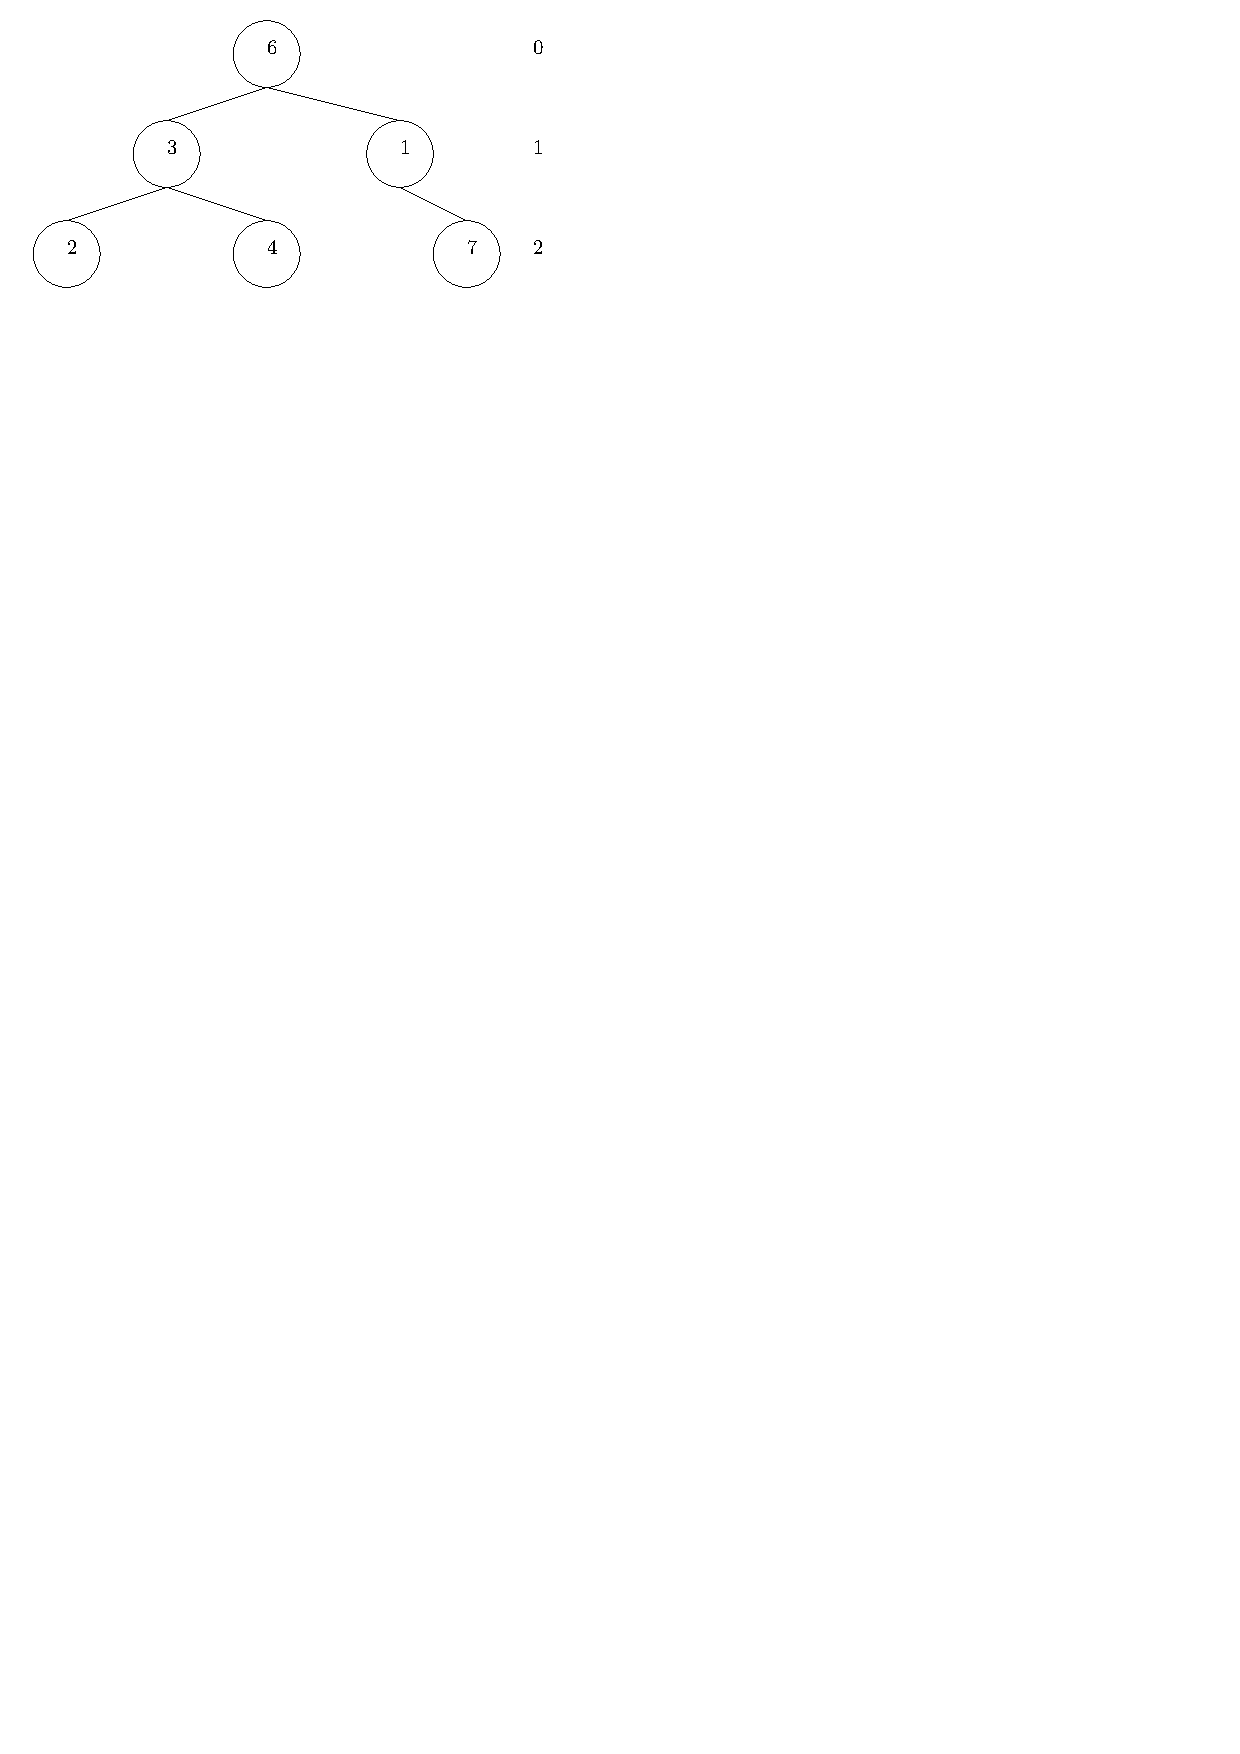
\includegraphics[width=\textwidth]{./A4Q2}
\caption{}
\label{fig:A4Q2}
\end{figure}
\end{enumerate}
\item
\begin{enumerate}
\item
Suppose that a graph G has no sources. Then every node in G has at least one other node connected to it. Consider the resulting forest from a DFS algorithm, in particular consider the root of each discovery tree. Every root must have either a back edge or a cross edge leading to it. If there is a back edge we are done there is a cycle. If there are no back edges and only cross edges we start at one root and follow down the discovery tree until we reach a cross edge to another discovery tree. We continue until we end up back at that root, and have therefore found the path of the cycle. 

I have shown that if G has no sources then it has a cycle. Therefore if G is acyclic, then it has at least one source.

\item
Note if G is acyclic then the tree resulting from deleting a node from G is also acyclic.

If G is acyclic then G has at least one source by the previous question. By the note above deleting a node also results in an acyclic graph which must also have at least one source. This will continue on until the graph is empty.

If G has a cycle, then if we isolate that cycle from the graph there are no sources within that cycle. Removing the nodes outside of the cycle will not result in creating sources within the cycle. So therefore source-deletion will delete everything from the graph except that cycle. Which means that at the end the graph will not be empty. 

Therefore G is acyclic if and only if source-deletion results in an empty graph.
\item My algorithm starts by finding all sources in G ($O(m + n)$) keeping track of all the sources in a linked list as well as a size variable. I then traverse the list, deleting all edges from each source and if appropriate add more sources to the end of the list and increment the size variable.
 ($O(m)$). When I reach the end of the list I compare the size variable to n, if they are equal there are no cycles. There for my algorithm runs in $O(m + n)$
 
 In the following code I assume that the linked lists I implement are iterable and therefore I can use a for loop.
 
 \begin{codebox}
 \Procname{$\proc{hasCycles}(n,E)$}
 \li $S \gets $Empty iterable linked list
 \li $\id{size} \gets 0$
 \li \For $i \in 1..n$
 \li \Do
 \li \For $e \in A[i]$
 \li \Do
 \li $I(e) \gets I(e) + 1$
 	\End
 	\End
 \li \For $i \in 1 \twodots n$
 \li \Do
 \li \If $I(i) = 0$
 \li \Then
 \li $\id{size} \gets \id{size} + 1$
 \li $\proc{Append}(S, i)$
 \End
 \End
 \li \For $i \in \id{S.value}$
 \li \Do
 \li \For $e \in \id{A[i].value}$
 \li \Do 
 \li $I(e) = I(e) - 1$
 \li \If $I(e) = 0$
 \li \Then
 \li $\id{size} \gets \id{size} + 1 $
 \li $\proc{Append}(S, e)$
 \End
 \End
 \End
 \li \If $\id{size} = n$
 \li \Then
 \li \Return $\const{False}$
 \End
 \li \Return $\const{True}$
 \end{codebox}
\end{enumerate}
\end{enumerate}
\end{document}